\documentclass[12pt,letterpaper]{article}
\usepackage{preamble}
\usepackage[brazil]{babel}
\usepackage[utf8]{inputenc}
\usepackage{enumitem}

%%%%%%%%%%%%%%%%%%%%%%%%%%%%%%%%%%%%%%%%%%
%%%% Edit These for yourself
%%%%%%%%%%%%%%%%%%%%%%%%%%%%%%%%%%%%%%%%%%
\newcommand\course{IA753}
\newcommand\hwnumber{2}
\newcommand\userID{Heitor S. Fernandes - RA: 074096}

\begin{document}
\centerline{\textbf{\Large Trabalho Computacional \hwnumber}}

\centerline{\text{ Linguagem utilizada: Python }}

\section*{Tarefa 1.}
\begin{enumerate}[label=(\alph*)]  %,leftmargin=!,labelindent=5pt]
    \item O sinal foi carregado a partir do arquivo \emph{signal.txt}. A frequência de amostragem ${f_s = 500 Hz}$ foi utilizada para calcular o tamanho do passo temporal: ${dt = 1/f_s = 0.002}$ segundos . A partir de ${dt}$ e do número de amostras ${N = 1000}$, foi criado um vetor tempo, indo de 0.000 a 19.998 segundos. O sinal no tempo pode ser visto na figura \ref{fig:1}, abaixo.
    
        \begin{figure}[H]
            \centering
            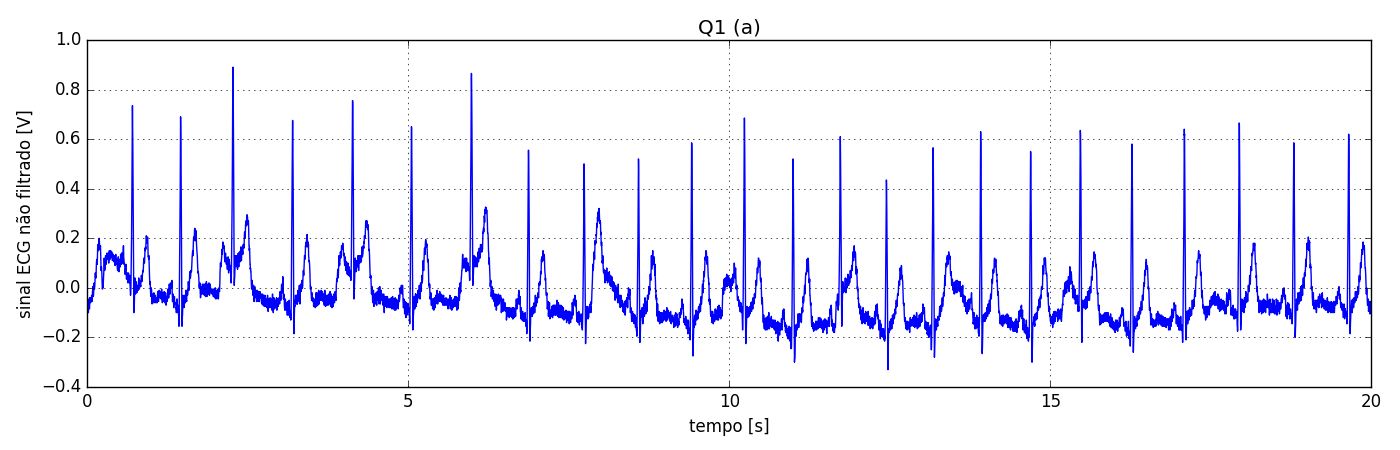
\includegraphics[width=15cm]{TC1/images/Q1_a_sinal_nfilt.png}
            \caption{Sinal de ECG em função do tempo.}
            \label{fig:1}
        \end{figure}

    \item
    Foi utilizado o comando \lstinline{np.fft.rfft} para obter a FFT do sinal (figura \ref{fig:2}). Outra maneira seria utilizar a FFT complexa (\lstinline{np.fft.fft}) e utilizar a apenas a parte real da resposta. O comando \lstinline{np.fft.rfftfreq} fornece as frequências de amostragem, porém em unidade adimensional. Para calibrar o eixo das abscissas em Hertz foi calculada a resolução espectral como o inverso do tempo se amostragem, isto é, ${df = {1/(dt*N)} = 0.05 Hz}$, e utilizado o número de amostras $N$.
    
    $${f_{Hz} = f_{adim}*df*N = {f_{adim} \over {dt*N}} *N = {f_{adim} \over dt}}$$
    
        \begin{figure}[H]
            \centering
            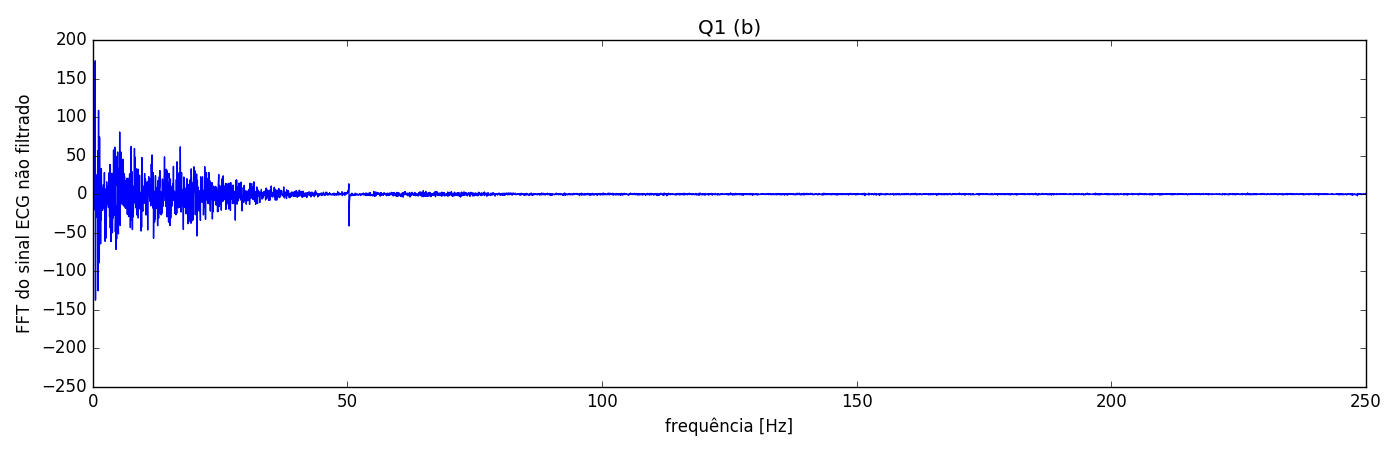
\includegraphics[width=15cm]{TC1/images/Q1_b_espectro_nfilt.png}
            \caption{Espectro do sinal de ECG.}
            \label{fig:2}
        \end{figure}
        
    \item
    O espectro possui componentes próximas a 50Hz, possivelmente devido à interferência da rede elétrica do local. São observadas, também, componentes em baixas frequências que podem estar relacionadas à respiração ou outros movimentos do indivíduo durante a aquisição do sinal e componentes em alta frequência, que podem estar relacionadas à detecção de sinais de EMG e ruídos causados pelos fios e pela interface entre a pele e os eletrodos.
    
    \item
    
    
\end{enumerate}

\section*{Tarefa 2}
Para criar os filtros foram utilizadas funções da biblioteca \lstinline{scipy.signal}.
\begin{enumerate}[label=(\alph*)]  %,leftmargin=!,labelindent=5pt]
    \item Filtro passa-baixas.
    
    (a.1)(a.2) O filtro passa-baixas foi projetado com as seguintes restrições: atenuação em 50Hz de 40dB (ou seja, faixa de rejeição iniciando em 50Hz), ordem máxima do filtro igual a 10 (para evitar instabilidade do filtro) e atenuação máxima de 3dB na faixa de passagem. Com estas restrições a faixa de passagem foi um resultado do projeto do filtro. Iterativamente, foi utilizada a função \lstinline{buttord} fixando-se a frequência da faixa de rejeição ($f_{stop}$) em 50Hz, a atenuação na faixa de passagem em 3dB e a atenuação na faixa de rejeição em 40dB. Desta maneira a frequência de corte máxima para obter um filtro de ordem máxima igual a 10 foi de $f_{pass} = 32Hz$.
    
    Então, foi utilizada a função \lstinline{butter} para gerar o filtro ButterWorth passa-baixas de ordem 10 e frequência de corte de 32Hz.
    
    (a.3) Função de transferência do filtro passa-baixas:
    
    $${Y(z) \over X(z)} = H(z) =
        {
        { \sum_{k=0}^{10}{b_k z^{-k}} }
        \over
        { \sum_{l=1}^{10}{a_l z^{-l}} }
        }
    $$
    
    Com os valores dos coeficientes $b_k$ e $a_l$ abaixo:
    
    \begin{table}
    \centering
    \begin{tabular}{lllll}
        $b_{0}$ & 3.39e-08 & \space & $a_{0}$ & 1.00 \\ 
        $b_{1}$ & 3.39e-07 & \space & $a_{1}$ & -7.43 \\ 
        $b_{2}$ & 1.53e-06 & \space & $a_{2}$ & 25.10 \\ 
        $b_{3}$ & 4.07e-06 & \space & $a_{3}$ & -50.73 \\ 
        $b_{4}$ & 7.12e-06 & \space & $a_{4}$ & 67.86 \\ 
        $b_{5}$ & 8.54e-06 & \space & $a_{5}$ & -62.73 \\ 
        $b_{6}$ & 7.12e-06 & \space & $a_{6}$ & 40.57 \\ 
        $b_{7}$ & 4.07e-06 & \space & $a_{7}$ & -18.12 \\ 
        $b_{8}$ & 1.53e-06 & \space & $a_{8}$ & 5.34 \\ 
        $b_{9}$ & 3.39e-07 & \space & $a_{9}$ & -0.94 \\ 
    \end{tabular}
    \end{table}
    
    Abaixo, a resposta em frequência do filtro:
            \begin{figure}[H]
            \centering
            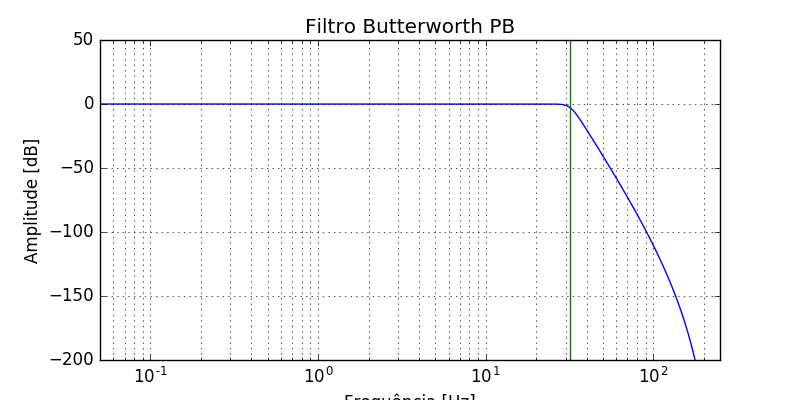
\includegraphics[width=15cm]{TC1/images/Q2_a3_PB_respfreq.png}
            \caption{Resposta em frequência do filtro passa-baixas.}
            \label{fig:3}
        \end{figure}
    
    
    Abaixo estão apresentados o espectro do sinal após o filtro passa-baixas (figura \ref{fig:4}) e um comparativo do sinal antes e depois do filtro (figura \ref{fig:5}), mostrando a atenuação das oscilações próximas a 50Hz.
    
        \begin{figure}[H]
            \centering
            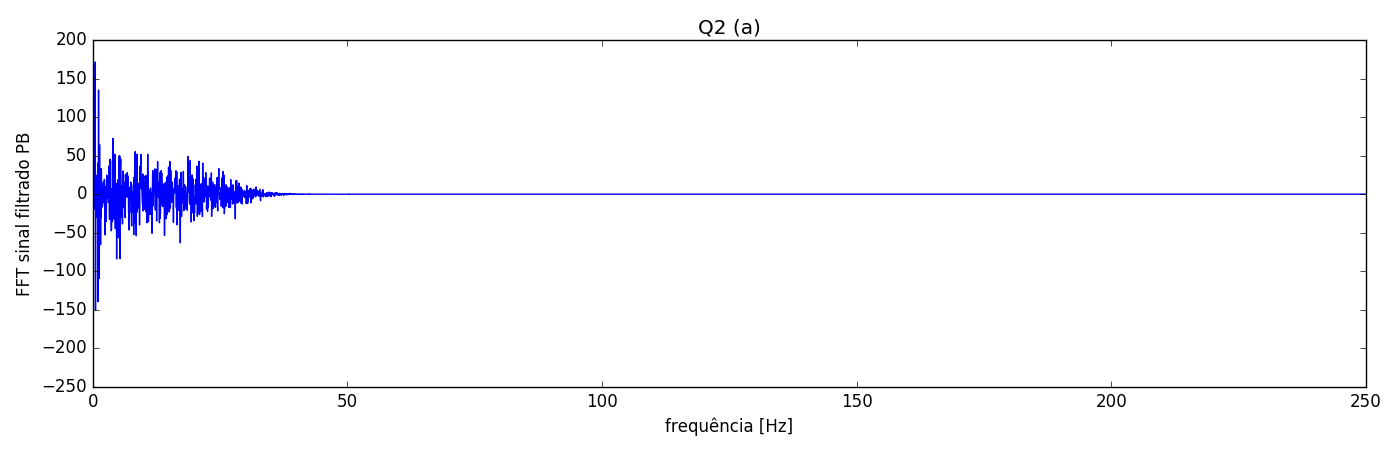
\includegraphics[width=15cm]{TC1/images/Q2_b_espectro_filt_PB.png}
            \caption{Espectro do sinal de ECG após filtro passa-baixas (freq. corte = 32Hz.}
            \label{fig:4}
        \end{figure}
    
        \begin{figure}[H]
            \centering
            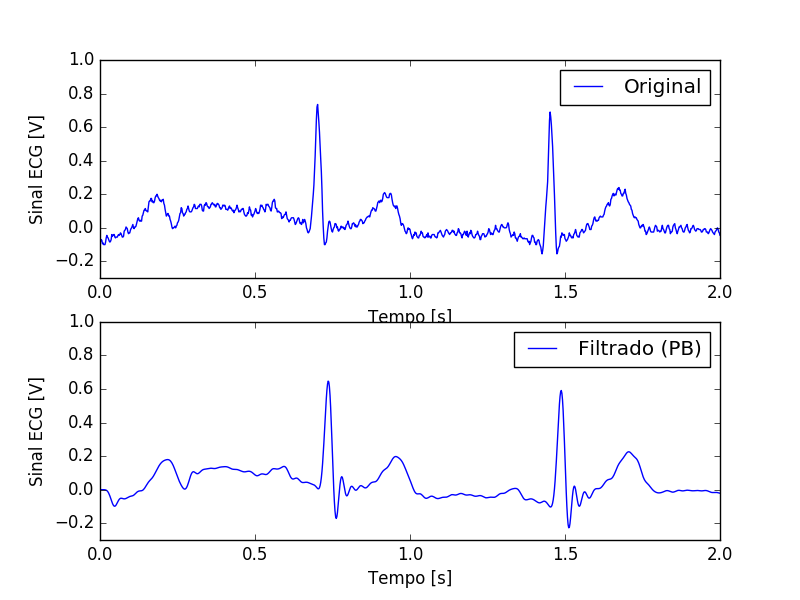
\includegraphics[width=15cm]{TC1/images/Q2_comparativo_orig_pb.png}
            \caption{Sinal ECG antes e depois do filtro passa-baixas (freq. corte = 32Hz.}
            \label{fig:5}
        \end{figure}
    
\newpage
    (a.4) Caso a frequência de corte escolhida para o filtro seja muito grande, as componentes perto de $50Hz$ serão menos atenuadas e para frequências de corte ainda menores que $32Hz$, aumenta-se a quantidade de informação que está sendo atenuada mas que poderia ser desejada para caracterizar o sinal de ECG.
    
    Abaixo, na figura \ref{fig:8}, mostra-se o sinal filtrado em três frequências de corte: $22Hz$, $32Hz$ (do filtro original) e $42Hz$.

        \begin{figure}[H]
            \centering
            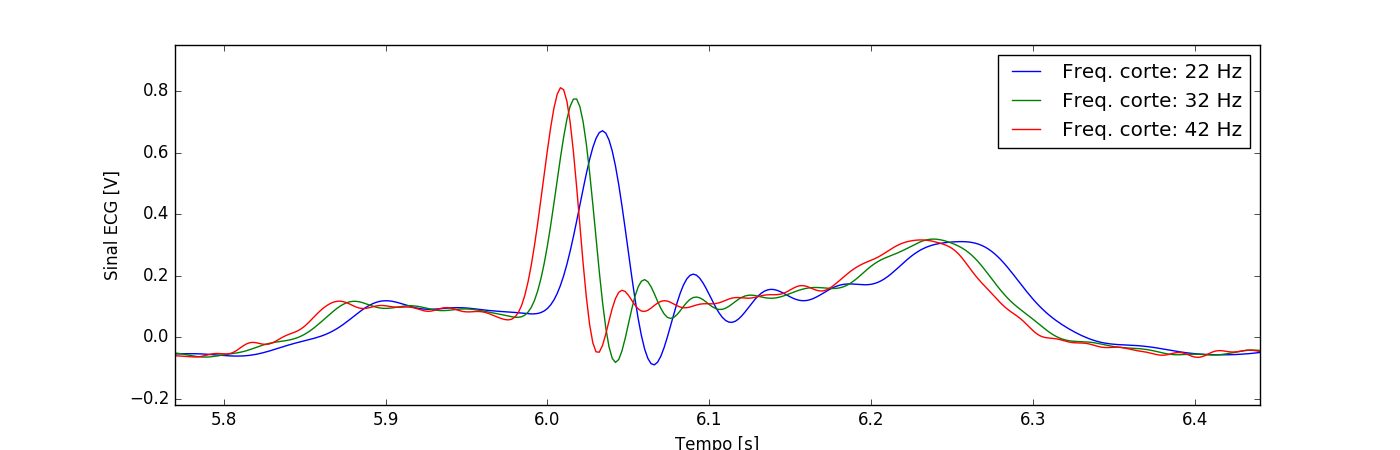
\includegraphics[width=15cm]{TC1/images/Q2a4_freqs_corte.png}
            \caption{Sinais filtrado em três frequências de corte distintas.}
            \label{fig:8}
        \end{figure}


     \item  Filtro passa-altas.
     
    (b.1)(b.2) Para o filtro passa-altas foi escolhida a frequência de corte de 0.5Hz para filtrar as flutuações da linha de base que possam estar relacionadas a respiração ou movimentações do sujeito durante a aquisição do sinal. O filtro foi projetado com atenuação mínima de 40dB na faixa de rejeição e de no máximo 3dB na faixa de passagem (acima de 0.5Hz). A ordem do filtro foi definida como 4, pois, com ordens a partir de 5 o filtro apresentava descontinuidades na resposta em frequência abaixo de 0.1Hz.
    
    Abaixo, a resposta em frequência do filtro passa-altas.
     
        \begin{figure}[H]
            \centering
            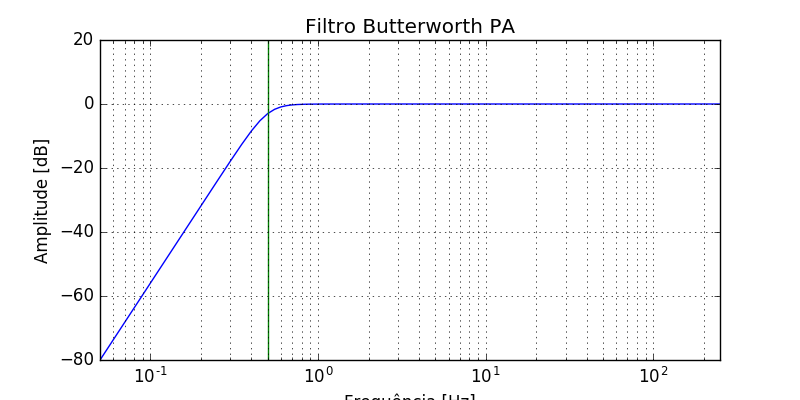
\includegraphics[width=15cm]{TC1/images/Q2_b_filtro_PA_respfreq.png}
            \caption{Resposta em frequência do filtro passa-altas (freq. corte = 0.5Hz).}
            \label{fig:9}
        \end{figure}
        
        
    (b.3) Função de transferência do filtro passa-altas:
    
    $${Y(z) \over X(z)} = H(z) =
        {
        { \sum_{k=0}^{4}{b_k z^{-k}} }
        \over
        { \sum_{l=1}^{4}{a_l z^{-l}} }
        }
    $$
    
    Com os valores dos coeficientes $b_k$ e $a_l$ abaixo:
    
    \begin{table}[H]
    \centering
    \begin{tabular}{lllll}
        $b_{0}$ &  0.9918 & \space & $a_{0}$ &  1 \\ 
        $b_{1}$ & -3.9672 & \space & $a_{1}$ & -3.9835 \\ 
        $b_{2}$ &  5.9509 & \space & $a_{2}$ &  5.9508 \\ 
        $b_{3}$ & -3.9672 & \space & $a_{3}$ & -3.9510 \\ 
        $b_{4}$ &  0.9918 & \space & $a_{4}$ &  0.9837 \\ 

    \end{tabular}
    \end{table}

    Nas figuras \ref{fig:10} e \ref{fig:11}, abaixo, estão apresentados o espectro do sinal após o filtro passa-altas e um comparativo do sinal antes e depois do filtro. É possível observar a atenuação em baixíssimas frequências e o ajuste das flutuações na linha-base.
    
        \begin{figure}[H]
            \centering
            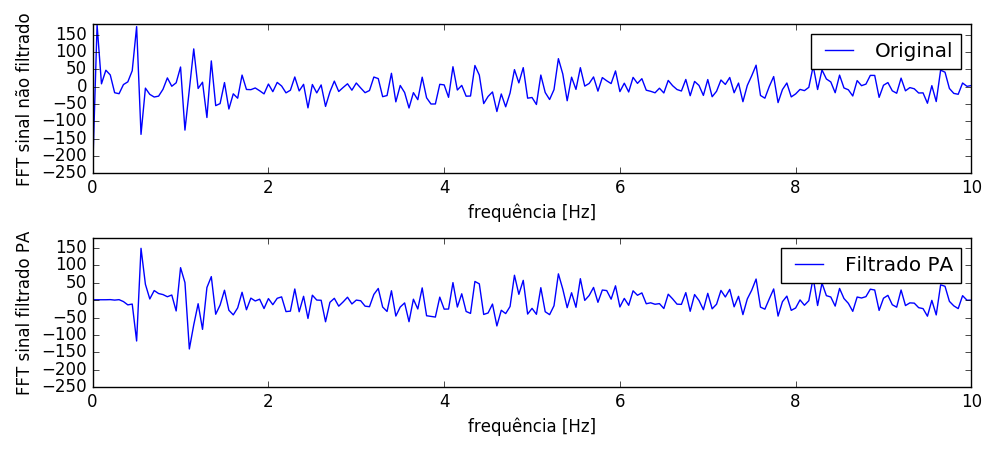
\includegraphics[width=15cm]{TC1/images/Q2_b_espectro_filt_PA_comparativo.png}
            \caption{Espectro do sinal de ECG após filtro passa-altas (freq. corte = 0.5Hz.}
            \label{fig:10}
        \end{figure}
    
        \begin{figure}[H]
            \centering
            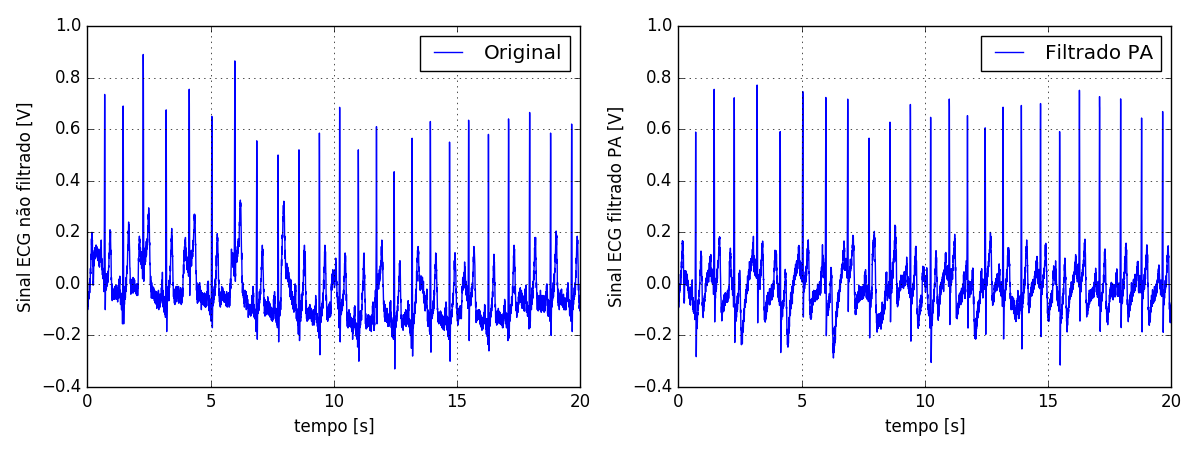
\includegraphics[width=15cm]{TC1/images/Q2_b_sinal_filt_PA.png}
            \caption{Comparativo do sinal ECG antes e depois do filtro passa-altas (freq. corte = 0.5Hz.}
            \label{fig:11}
        \end{figure}
    
\newpage
    (b.4) Caso a frequência de corte fosse menor, parte da flutuação da linha de base não seria removida, porém, caso a frequência de corte fosse mais que 0.5, haveria uma distorção ainda maior no espectro de baixas frequências, podendo haver perda significativa de informação.
    
    Abaixo, mostra-se o sinal filtrado em três frequências de corte: $0.1Hz$, $0.5Hz$ (do filtro original) e $5.0Hz$.  Observa-se que um filtro com frequência de corte muito baixa como 0.1Hz ainda deixa presente algumas flutuações de baixa frequência. O sinal filtrado com passa-altas a 5HZ, por sua vez, causa uma deformação no sinal, o que não é observado no sinal filtrado a 0.5Hz.

        \begin{figure}[H]
            \centering
            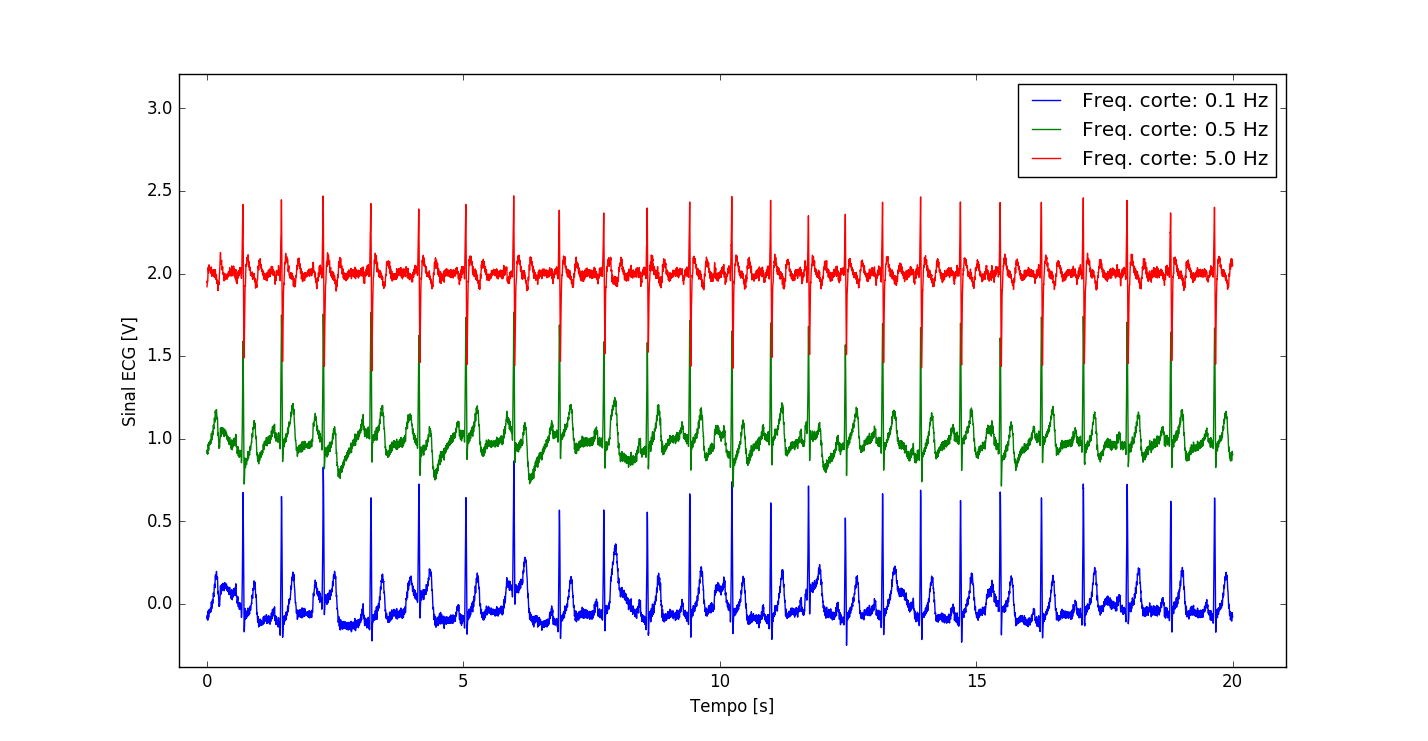
\includegraphics[width=15cm]{TC1/images/Q2b4_freqs_corte.png}
            \caption{Sinais filtrado em três frequências de corte distintas. Os sinais filtrados a 0.5Hz (linha verde) e a 0.1Hz (linha vermelha) estão deslocados em 1V e 2V, respectivamente, para melhor observação de seus efeitos. }
            \label{fig:12}
        \end{figure}

    \item Filtro Notch.
    
    Para implementar o filtro Notch foi utilizada a função \lstinline{iirnotch}, também da biblioteca \lstinline{scipy.signal}.
    
    Para utilizar esta função entra-se com a frequência de filtragem e o fator de qualidade. Um favor de qualidade de 25 foi suficiente para ter atenuação de 40dB na frequência de 50.3Hz.
    
    Abaixo, a resposta em frequência do filtro Notch projetado.
    
        \begin{figure}[H]
            \centering
            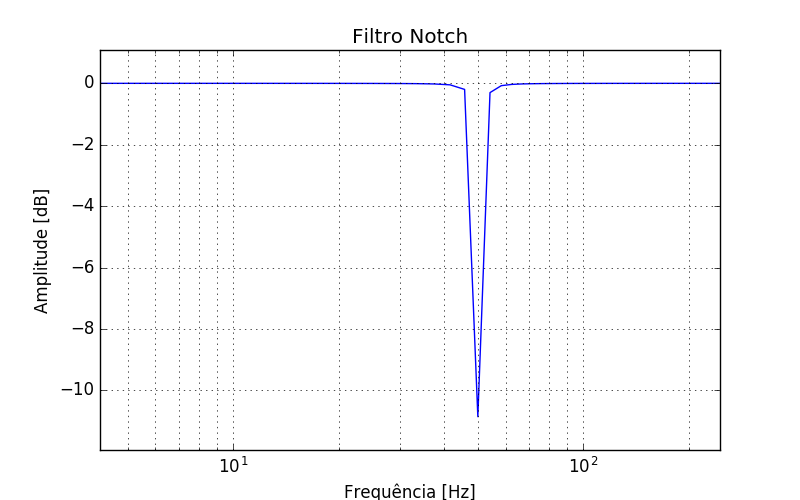
\includegraphics[width=15cm]{TC1/images/Q2c_Notch_respfreq.png}
            \caption{Resposta em frequência do filtro Notch.}
            \label{fig:13}
        \end{figure}

    Na figura \ref{fig:15}, abaixo, é possível verificar o efeito do filtro Notch no sinal original.
    
        \begin{figure}[H]
            \centering
            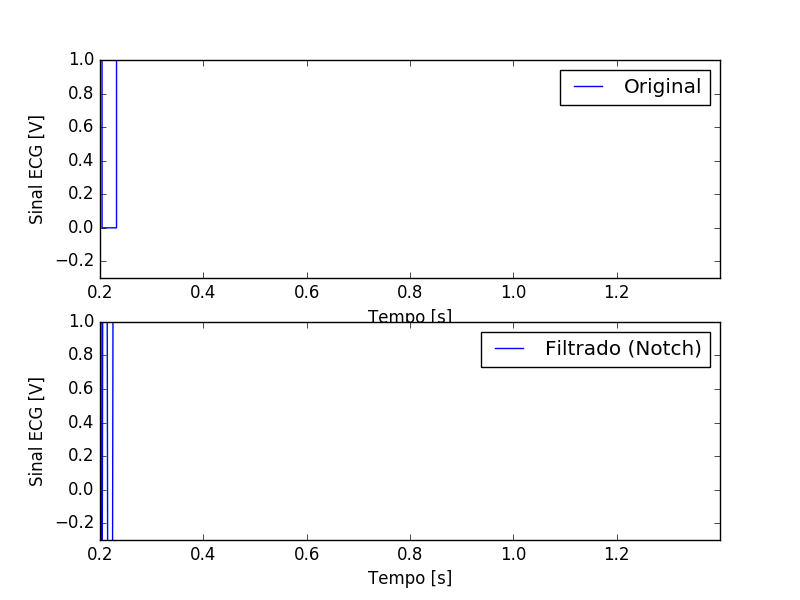
\includegraphics[width=15cm]{TC1/images/Q2c_comparativo_orig_notch.png}
            \caption{Sinal original comparado com o sinal após filtragem do tipo Notch.}
            \label{fig:15}
        \end{figure}
    
    
    \item Combinação de filtros.
    
    Foi decidido manter o filtro passa-altas para remover as flutuações em baixa frequência. Para eliminar as componentes excessivas próximas de 50Hz sem perder informações do sinal em frequências altas, foi utilizado o filtro Notch em 50.3Hz. Então, foi incluído um filtro passa-baixas com faixa de transição entre 80Hz e 120Hz, para filtrar componentes de frequências muito altas.
    
    Abaixo, nas figuras \ref{fig:16}, \ref{fig:17} e \ref{fig:18} é possível observar o efeito do filtro sobre o sinal no tempo e na frequência. Houve diminuição da flutuação da linha de base, remoção das frequências próximas a 50Hz e atenuação de frequências altíssimas.
    
        \begin{figure}[H]
            \centering
            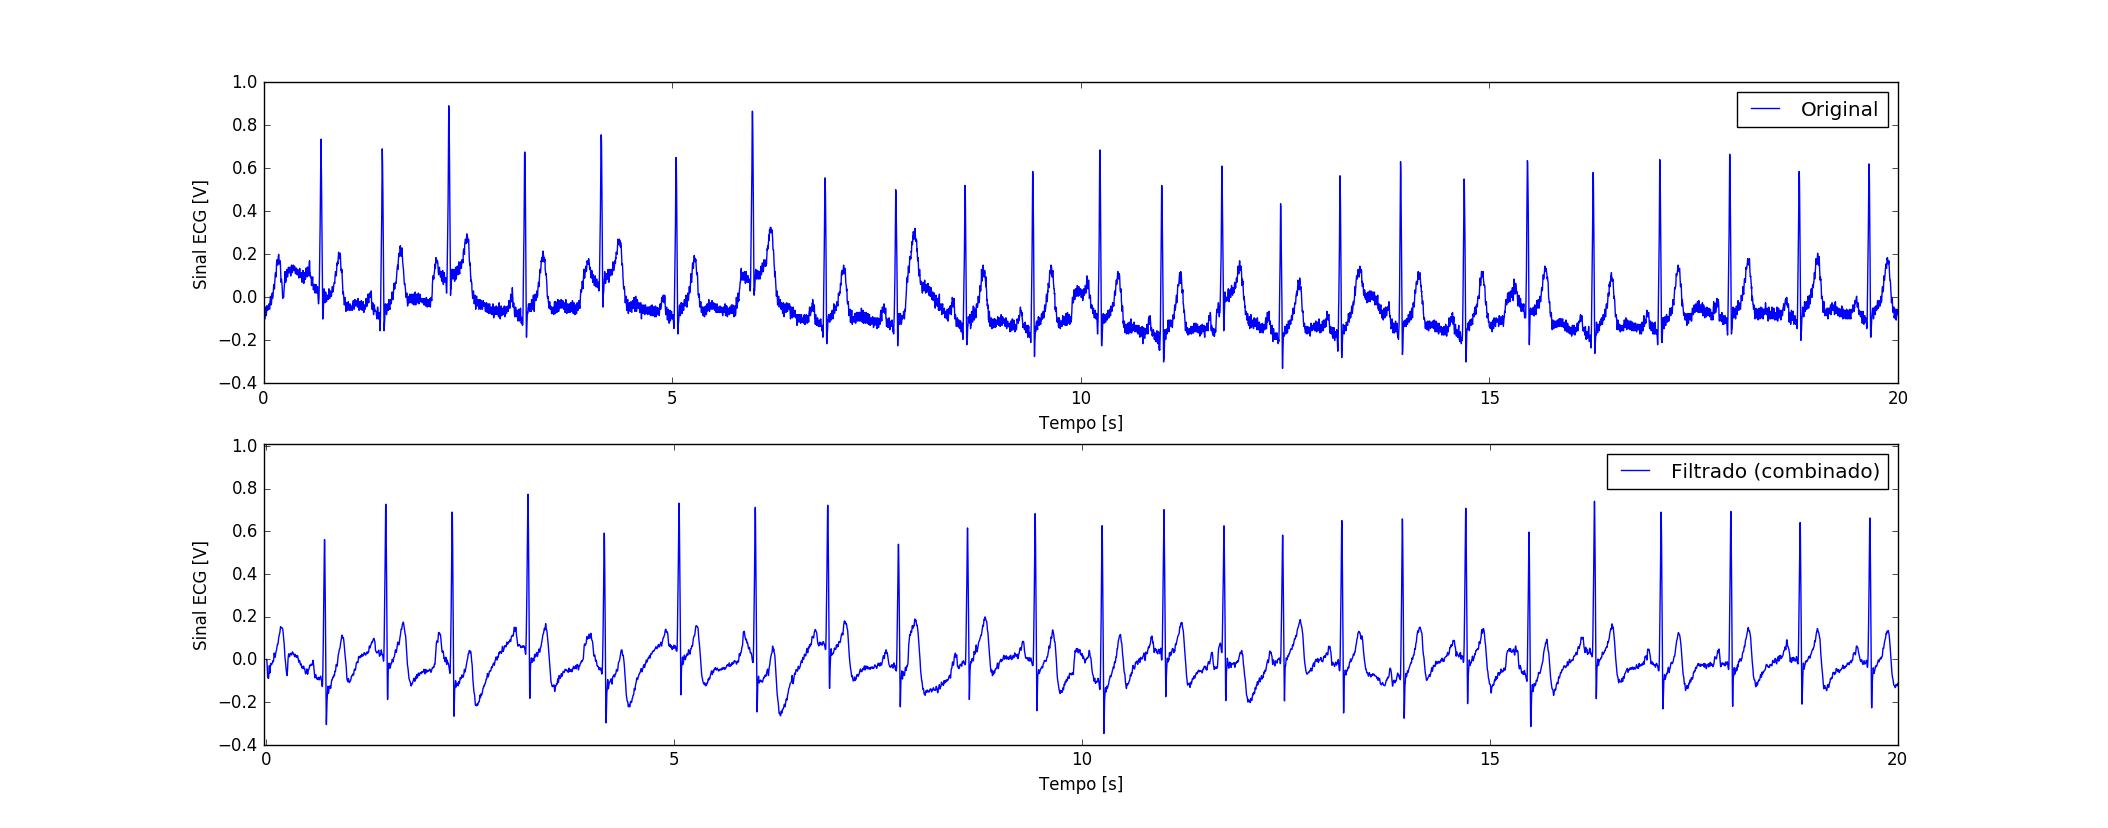
\includegraphics[width=15cm]{TC1/images/Q2d_comb_whole.png}
            \caption{Sinal original comparado com o sinal após filtragem combinada.}
            \label{fig:16}
        \end{figure}
        \begin{figure}[H]
            \centering
            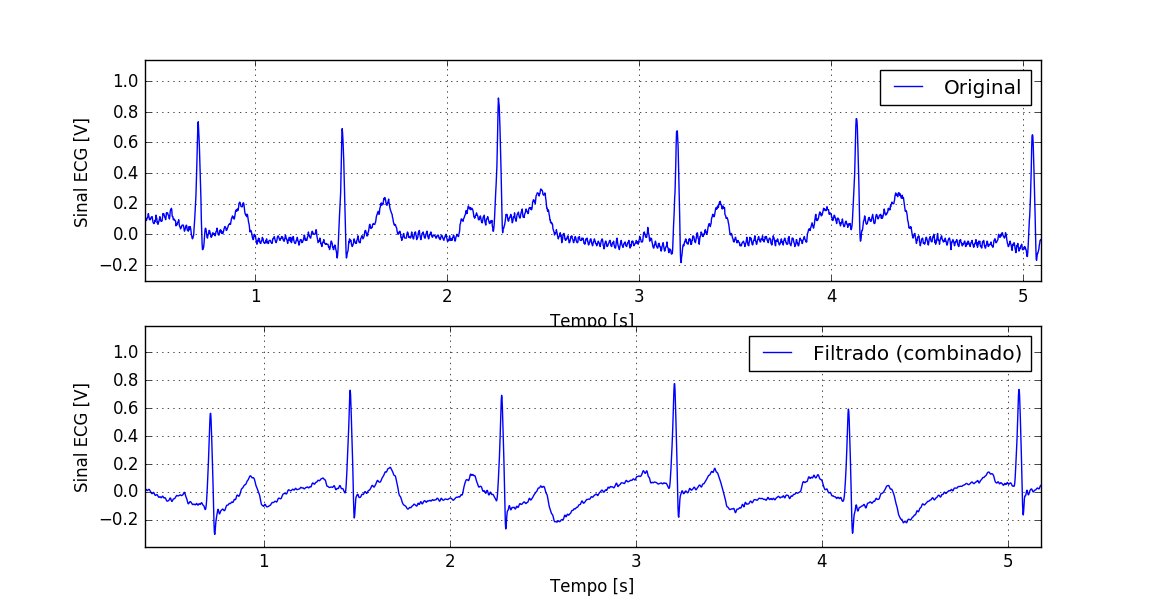
\includegraphics[width=15cm]{TC1/images/Q2d_comb_1-5seg.png}
            \caption{Sinal original comparado com o sinal após filtragem combinada, entre 1 e 5 segundos.}
            \label{fig:17}
        \end{figure}
        \begin{figure}[H]
            \centering
            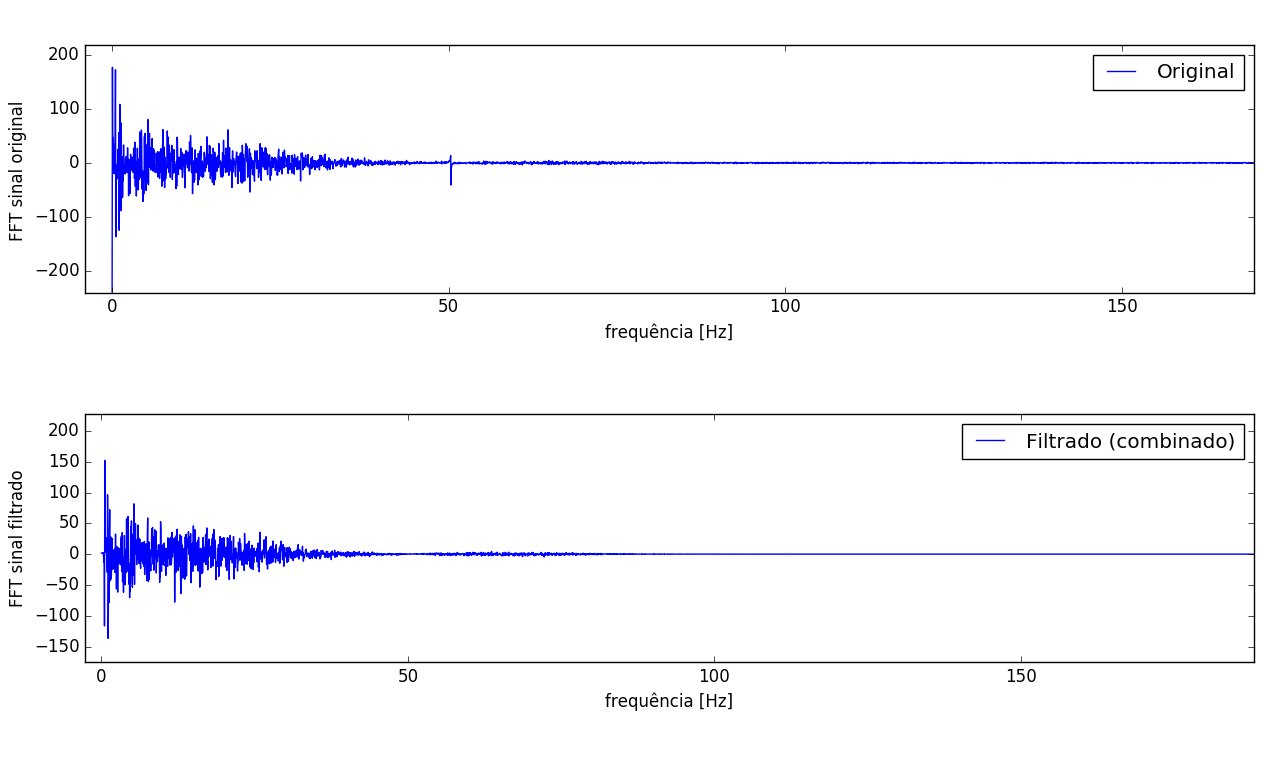
\includegraphics[width=15cm]{TC1/images/Q2d_comb_espectro_comparado.png}
            \caption{Espectro do sinal original comparado com o do sinal após filtragem combinada.}
            \label{fig:18}
        \end{figure}
    
\end{enumerate}


\section*{Questão 3. Estimar frequência instantânea.}
\begin{enumerate}[label=(\alph*)]  %,leftmargin=!,labelindent=5pt]
    \item Para identificar os picos do sinal de ECG filtrado foram verificados os pontos no sinal maiores que 0.3V que fossem, simultaneamente, maiores que o ponto imediatamente antes e maiores que o ponto imediatamente depois. Isto é:
    
    $signal[n]$ é um pico se $signal[n-1] < signal[n] > signal[n+1] , n = 2,3,..,N-1$
    
    Com N sendo o número de amostras do sinal. Abaixo, o sinal com os picos identificados.
    
        \begin{figure}[H]
            \centering
            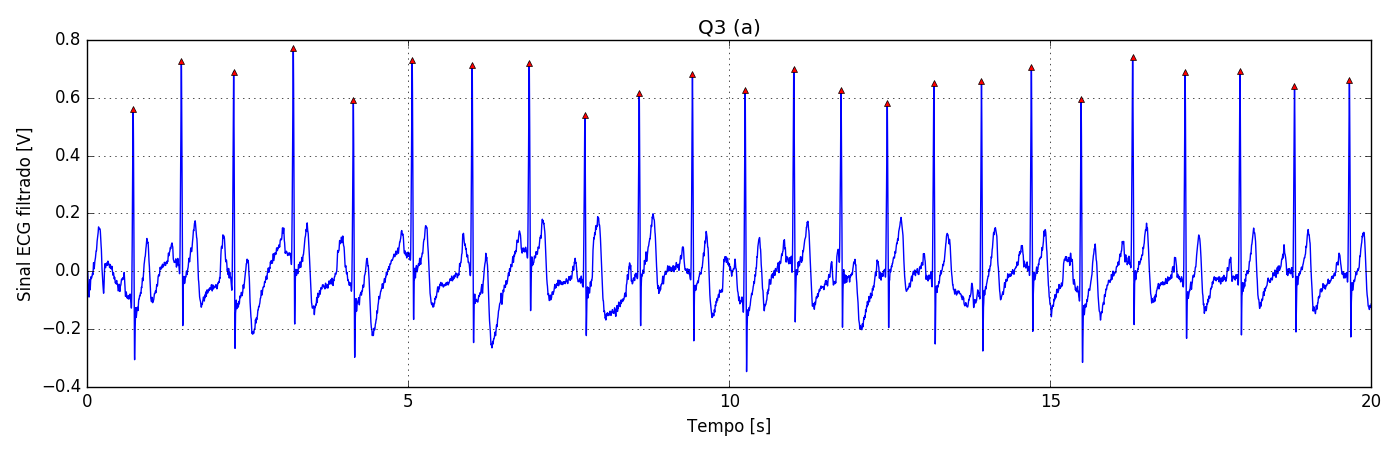
\includegraphics[width=15cm]{TC1/images/Q3a.png}
            \caption{Sinal filtrado com os picos identificados (triângulos vermelhos).}
            \label{fig:19}
        \end{figure}
    
    \item O trem de impulsos foi criado a partir de um vetor de zeros de mesmo tamanho que o sinal para que a frequência de amostragem seja igual à do sinal. Então, nos instantes onde ocorrem os picos, os zeros foram substituídos pelo valor $1/{dt}$, representando o impulso discreto.
    
        \begin{figure}[H]
            \centering
            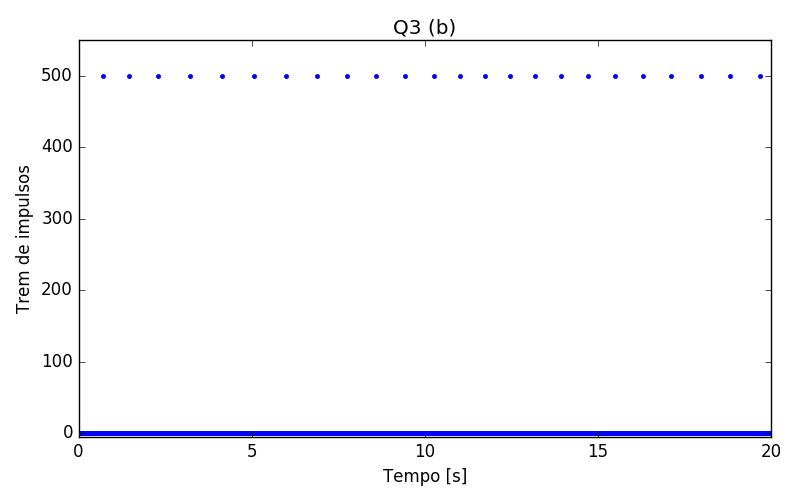
\includegraphics[width=.9\textwidth]{TC1/images/Q3b.png}
            \caption{Trem de impulsos.}
            \label{fig:20}
        \end{figure}
        
    \item A janela foi criada como um vetor com $w$ valores iguais a $1/w$. A convolução foi feita usando a função \lstinline{np.convolve}.
    
    Para uma janela muito pequena, a convolução irá mostrar pulsos nos instantes dos impulsos, como é o caso de $w = 100$, visto na figura \ref{fig:21}. Por outro lado, caso a janela seja muito grande, como $w = 5000$, a convolução irá apresentar um perfil quase triangular, como pode ser visto na figura \ref{fig:22}. No entanto, uma janela bem ajustada resulta em um convolução que com poucos pontos passa a oscilar em torno do que seria a frequência média estimada, como pode ser visto na figura \ref{fig:23}, com $w = 1200$.
        \begin{figure}[H]
            \centering
            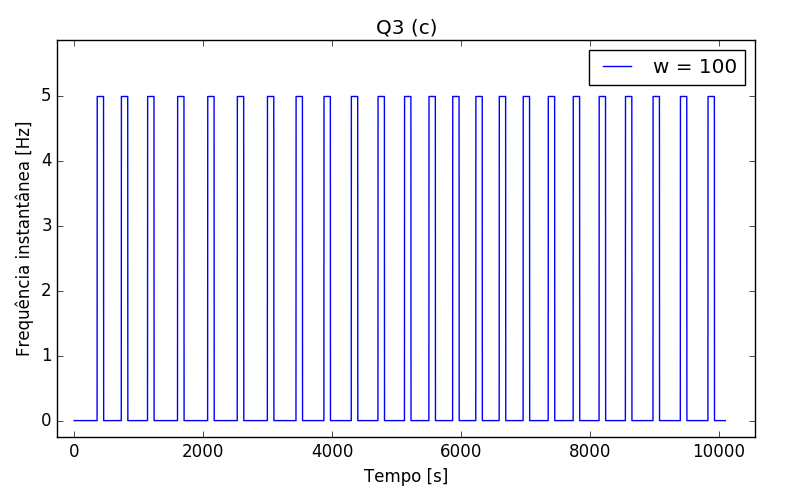
\includegraphics[width=.9\textwidth]{TC1/images/Q3c_w_toosmall.png}
            \caption{Estimação de frequência instantânea por convolução com janela muito pequena.}
            \label{fig:21}
        \end{figure}
        \begin{figure}[H]
            \centering
            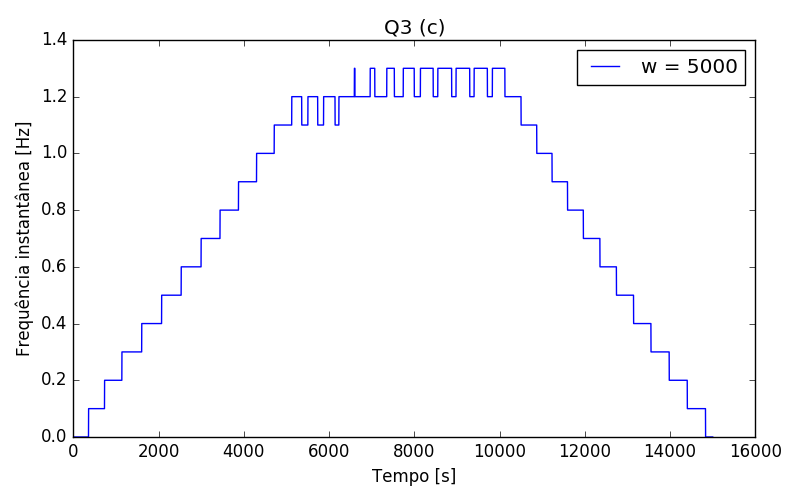
\includegraphics[width=.9\textwidth]{TC1/images/Q3c_w_toobig.png}
            \caption{Estimação de frequência instantânea por convolução com janela muito grande.}
            \label{fig:22}
        \end{figure}
        \begin{figure}[H]
            \centering
            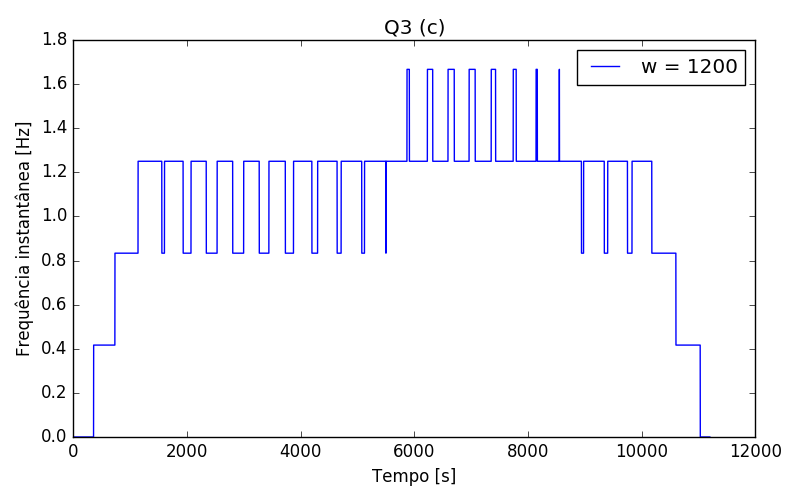
\includegraphics[width=.9\textwidth]{TC1/images/Q3c.png}
            \caption{Estimação de frequência instantânea por convolução com janela adequada.}
            \label{fig:23}
        \end{figure}
\end{enumerate}

\end{document}
